\chapter{Desarrollo del entorno base}\label{ch:desarrollo-del-entorno-base}


\section{Interfaz de usuario}\label{sec:interfaz-de-usuario}

La interfaz de \textit{JAMS} es muy similar a las interfaces que presentan los \textit{IDEs} modernos.
Todas las herramientas están encapsuladas en $nodos$.
Cada nodo se puede desplegar en los laterales del editor.
Más concretamente, se pueden desplegar dos nodos por cada lado del editor.

\begin{figure}[H]
    \centering
    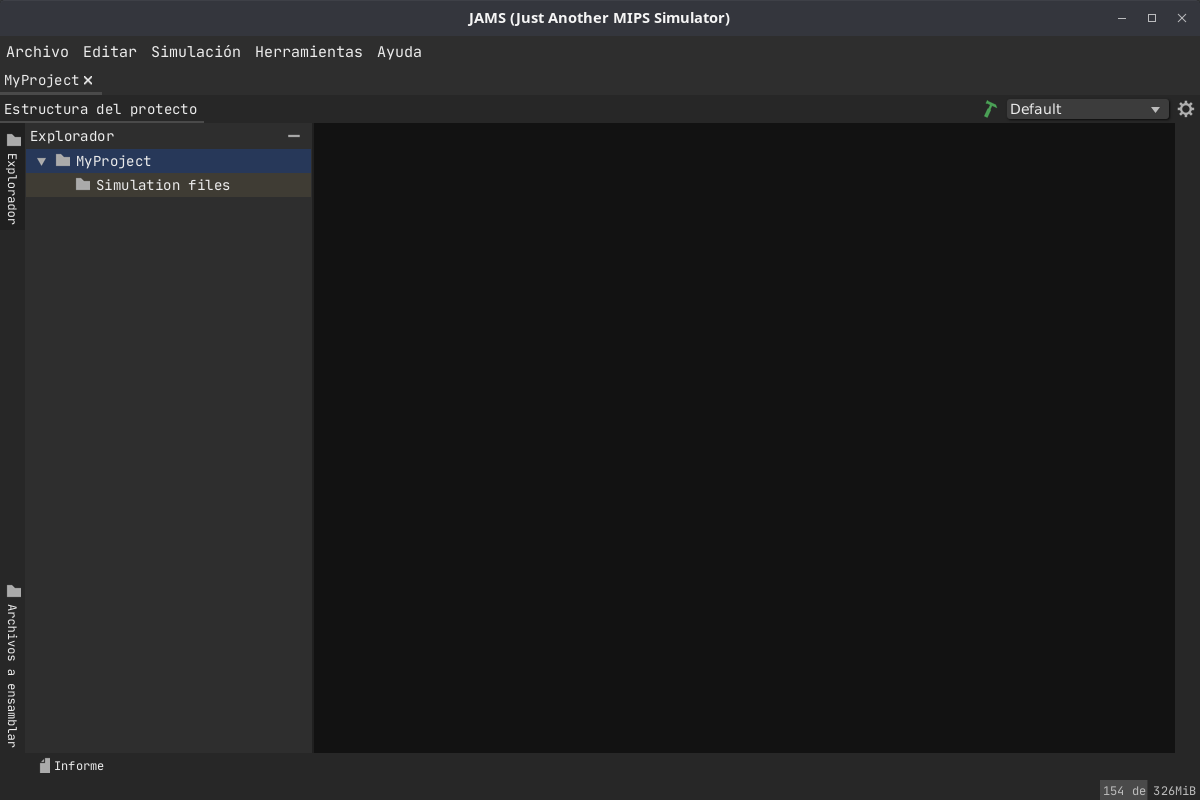
\includegraphics[width=0.8\textwidth]{images/base/jams-basic}
    \caption{\textit{Editor de \textit{JAMS} en su forma más básica}}
    \label{fig:jams-basic}
\end{figure}

Los nodos también se pueden configurar para que se desplieguen
en una ventana aparte.
Esto permite poder desplegar un número indefinido de nodos al mismo tiempo.
El modo de despliegue se puede configurar presionando el botón secundario sobre
el botón del nodo.

\begin{figure}[H]
    \centering
    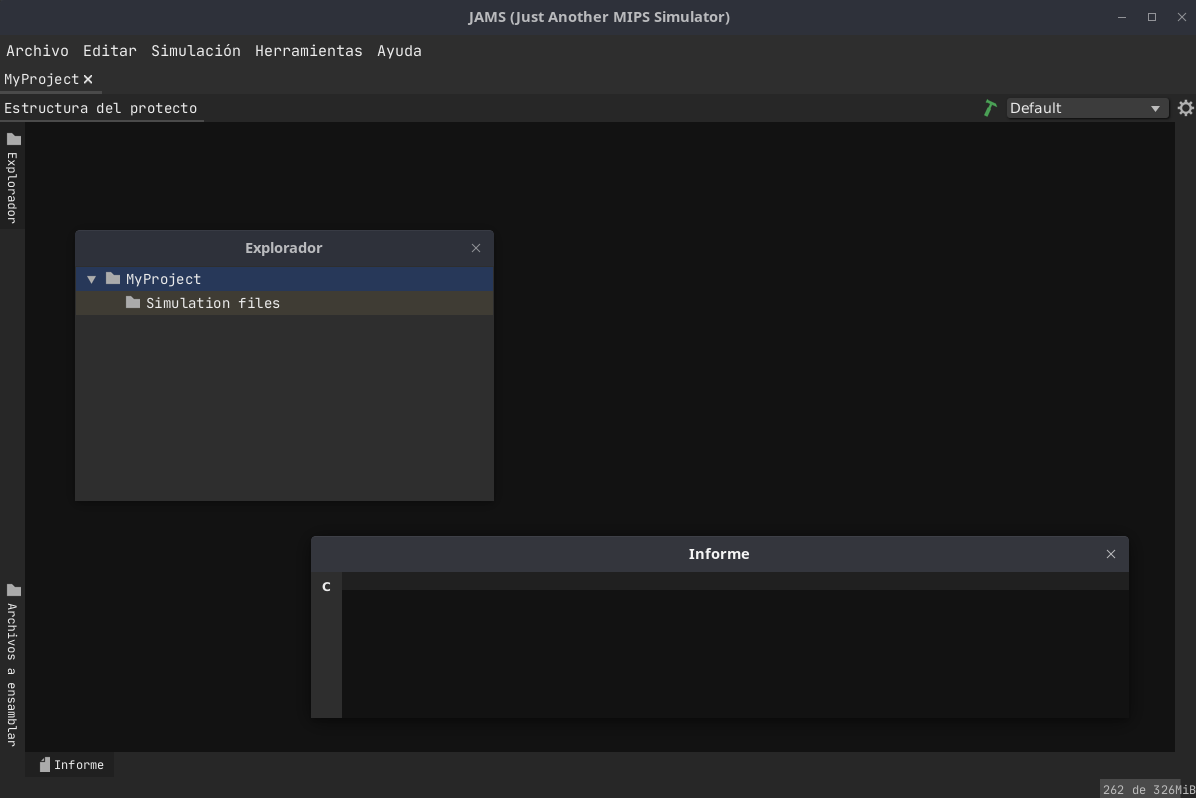
\includegraphics[width=0.8\textwidth]{images/base/jams-windows}
    \caption{\textit{Editor de \textit{JAMS} con ventanas desplegadas}}
    \label{fig:jams-windows}
\end{figure}

\subsection{Menú superior}\label{subsec:menu-superior}

El menú superior de \textit{JAMS} funciona de manera idéntica
a cualquier otro programa.
Por defecto existen cinco secciones:
\begin{itemize}
    \item \textbf{Archivo}: permite crear o abrir nuevos proyectos, además de
    acceder a la configuración.
    \item \textbf{Editar:} permite acceder a los comandos del editor de texto.
    \item \textbf{Simulación:} permite acceder a los comandos de simulación.
    \item \textbf{Herramientas:} permite habilitar o deshabilitar nodos.
    \item \textbf{Ayuda:} permite acceder a ayuda sobre \textit{JAMS}.
\end{itemize}

\subsection{Proyectos abiertos}\label{subsec:proyectos-abiertos}

Los proyectos abiertos aparecen justo debajo del menú superior.
Cada proyecto está representado por una pestaña, lo que facilita alternar entre
proyectos abiertos.
Si se cierran todos los proyectos, \textit{JAMS} cerrará el editor y trasladará
al usuario a la ventana de inicio.

Los proyectos presentan una lista de pestañas con todas las secciones
que tienen abiertas.
Normalmente, la primera pestaña representa el editor del proyecto, mientras que
las siguientes representan las simulaciones que el usuario vaya creando.

\begin{figure}[H]
    \centering
    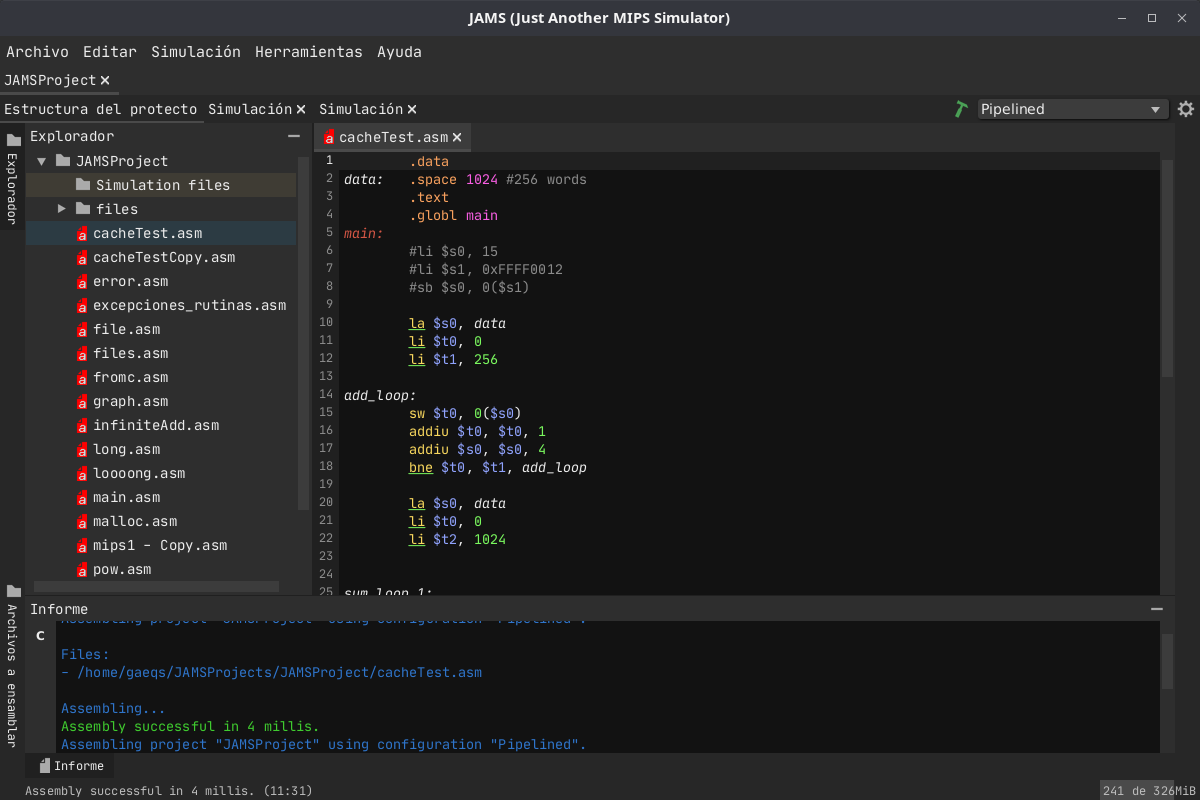
\includegraphics[width=0.8\textwidth]{images/base/jams-sections}
    \caption{\textit{Editor de \textit{JAMS} con varias simulaciones creadas}}
    \label{fig:jams-sections}
\end{figure}

Cada sección tiene una \textbf{barra de herramientas} propia.
Esta barra está situada a la izquierda de la lista de secciones, y permite
ejecutar acciones relacionadas con la sección actual.

\subsection{Barra inferior}\label{subsec:barra-inferior}

La barra inferior del editor es común a todas las secciones.
En esta, se informa del último mensaje escrito en el \textbf{informe}.
A la izquierda también se muestra la memoria que está usando actualmente
\textit{JAMS}.
Al estar creada la aplicación en \textit{Java}, esta utiliza un recolector
de basura.
Se puede forzar el paso del recolector de basura pulsando el panel que informa
sobre el uso de memoria.

\subsection{Ventana principal}\label{subsec:ventana-principal}

Si \textit{JAMS} no tiene ningún proyecto que mostrar, se mostrará la ventana
principal.
En esta ventana se pueden encontrar cuatro apartados:
\begin{itemize}
    \item \textbf{Proyectos:} en este apartado se encuentran los proyectos más
    recientes.
    También se puede abrir un proyecto ya existente.
    \item \textbf{Nuevo proyecto:} este apartado permite crear nuevos proyectos.
    Un componente puede añadir su propio creador de proyectos.
    \item \textbf{Configuración:} muestra la ventana de configuración.
    Permite configurar \textit{JAMS} antes de abrir un proyecto.
    \item \textbf{Acerca de:} muestra información básica sobre \textit{JAMS}.
\end{itemize}

\begin{figure}[H]
    \centering
    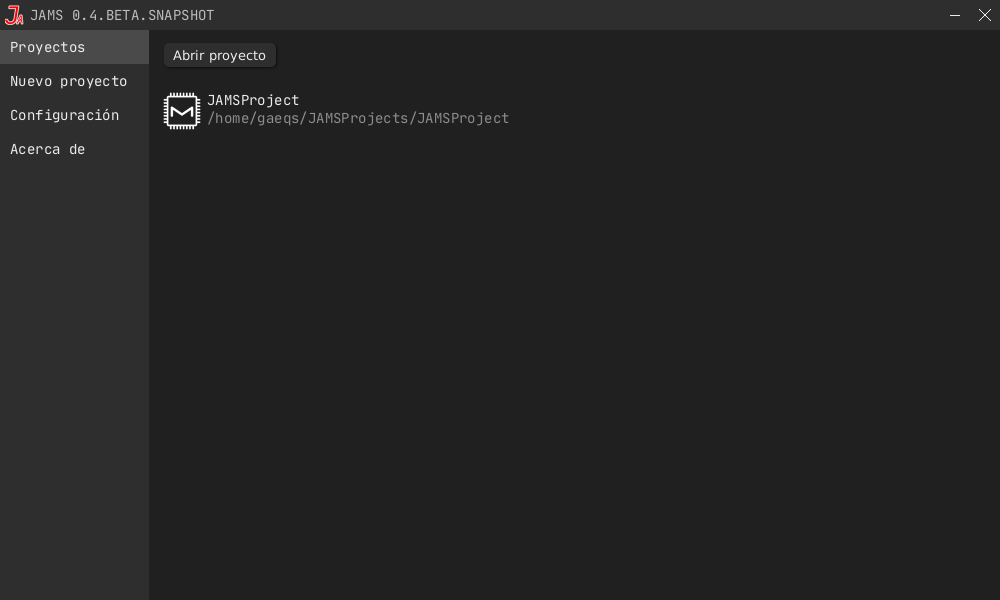
\includegraphics[width=0.8\textwidth]{images/base/jams-main-projects}
    \caption{\textit{Ventana principal mostrando los proyectos recientes}}
    \label{fig:jams-main-projects}
\end{figure}

\begin{figure}[H]
    \centering
    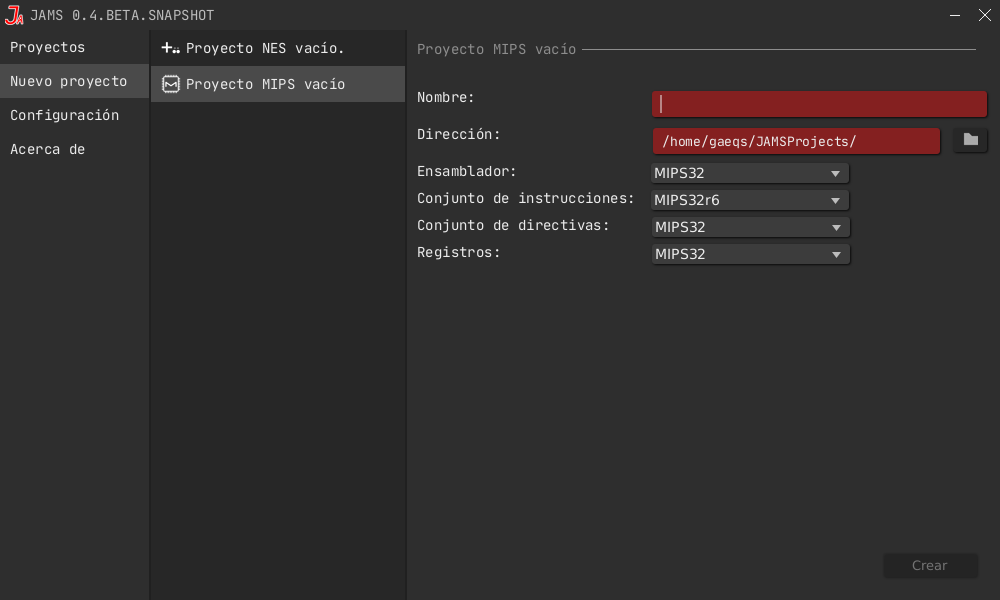
\includegraphics[width=0.8\textwidth]{images/base/jams-main-new-project}
    \caption{\textit{Ventana de creación de nuevos proyectos}}
    \label{fig:jams-main-new-project}
\end{figure}


\section{Idiomas}\label{sec:idiomas}

Igual que cualquier aplicación moderna, \textit{JAMS} presenta un sistema de
localización basado en paquetes de idiomas.
Cualquier usuario o componente puede crear un paquete que añada
o modifique un idioma.
El sistema de idiomas utiliza el estándar \textit{Unicode}, lo que permite
a los idiomas usar caracteres especiales en sus mensajes.

\subsection{Estructura de un paquete}\label{subsec:estructura-de-un-paquete}

Un paquete de idiomas es una carpeta o un archivo comprimido
que contienen un archivo \textbf{language.json}
y varios archivos \textit{YAML}\cite{YAML}.
Esta carpeta o archivo estará situado dentro de un componente
o dentro de la carpeta \textbf{\textasciitilde/JAMS/languages}.
Un ejemplo de un archivo \textbf{language.json} sería el siguiente:

\begin{lstlisting}[frame=single,label={lst:language.json}]
{
  "name": "English",
  "priority": 0,
  "files": [
    "actions.yml",
    "configuration.yml",
    "directives.yml"
  ]
}
\end{lstlisting}

Dentro de este archivo se encuentran los siguientes parámetros:
\begin{itemize}
    \item \textbf{name:} es el nombre del idioma.
    Este nombre es el que será mostrado al usuario
    y actúa como identificador del idioma.
    \item \textbf{files:} son los archivos \textit{YAML} que componen el paquete.
    \item \textbf{priority:} es la prioridad del paquete si existen varios
    paquetes para el mismo idioma.
    Cuanto más alto sea el número, más prioridad tiene el paquete.
    Esta propiedad es opcional y por defecto toma el valor 0.
\end{itemize}

Los archivos \textit{YAML} pueden estar en carpetas dentro del paquete,
y deben estar definidos en el archivo \textbf{language.json} con una
dirección relativa a la raíz del paquete.
Un ejemplo de archivo \textit{YAML} sería el siguiente:

\begin{lstlisting}[frame=single,label={lst:interface.yml}]
START_TITLE: JAMS {VERSION}
START_PROJECTS: Projects
START_NEW_PROJECT: New project
START_ABOUT: About
BOTTOM_BAR_MEMORY: '{USED} of {TOTAL}MiB'
BOTTOM_BAR_MEMORY_TOOLTIP: Click to execute the garbage collector.
\end{lstlisting}

\subsection{Extensiones}\label{subsec:idiomas-extensiones}

Puede existir el caso donde varios paquetes hagan referencia al mismo idioma.
Este problema de colisión se soluciona gracias a las extensiones.
Un paquete actúa siempre como una extensión de un idioma.
Esta extensión tiene una prioridad que se define en el archivo
\textbf{language.json} del paquete.
Si dos extensiones tienen la misma prioridad, el orden se resuelve
por orden de creación de la extensión, siendo el último en ser creado
el que tenga más prioridad.
El mensaje ligado a un identificador será el de la extensión con más prioridad
que contenga un mensaje ligado al identificador.
Gracias a este pequeño sistema de extensiones, los usuarios podrán crear modificaciones
y los componentes podrán añadir nuevos mensajes.

\subsection{Instalación y selección de un idioma}\label{subsec:instalacion-y-seleccion-de-un-idioma}

Los usuarios pueden instalar un paquete de idioma arrastrando la carpeta o
archivo comprimido que lo contiene dentro de la carpeta \textbf{\textasciitilde/JAMS/languages}.
Una vez hecho esto, \textit{JAMS} mostrará los cambios realizados por el paquete
de idioma.
Si el paquete de idioma contiene un idioma nuevo, el usuario podrá seleccionarlo
desde la configuración.

\textit{JAMS} necesita que dos idiomas estén seleccionados al mismo tiempo:
el \textbf{idioma a mostrar} y el \textbf{idioma de respaldo}.
El idioma de respaldo se usará cuando el idioma a mostrar no defina un mensaje
necesario por la aplicación.
El usuario puede cambiar tanto el idioma a mostrar como el idioma de respaldo.
Cuando un idiomas es eliminado y este está seleccionado, \textit{JAMS}
buscará el idioma más adecuado para reemplazarlo.

El cambio de idioma, al igual que el resto de los parámetros de configuración,
tienen un efecto \textbf{instantáneo} en la aplicación, por lo que no es necesario
reiniciar la aplicación para que el cambio de idioma tenga efecto.


\section{Temas}\label{sec:temas}

Los temas de JAMS funcionan de la misma manera que el estilo de una página web:
mediante archivos \textit{CSS}\cite{CSS}.
\newODR{El }funcionamiento de los temas es muy similar al funcionamiento de los idiomas:
los temas son empaquetados en una carpeta o archivo comprimido,
con un archivo \textit{JSON} que actúa como punto de entrada (\textbf{theme.json})
y un conjunto de archivos \textit{CSS}.

A diferencia de los idiomas, un desarrollador que implemente nuevos
nodos a la escena de \textit{JAMS} no require gestionar ningún aspecto
de los temas: el tema que el usuario tenga seleccionado será implementado
de manera transparente gracias al sistema de temas de \textit{JavaFX}.

\subsection{Estructura}\label{subsec:estructura}

El archivo \textbf{theme.json} define el nombre y los archivos
\textit{CSS} incluidos en el tema.
Un ejemplo de archivo theme.json sería el siguiente:
\begin{lstlisting}[frame=single,label={lst:theme.json}]
{
  "name": "Light Theme",
  "dependencies": ["Other Theme"],
  "files": [
    "extra.css"
  ]
}
\end{lstlisting}

Un archivo \textbf{theme.json} presenta los siguientes parámetros:
\begin{itemize}
    \item \textbf{name:} es el nombre del tema.
    Este nombre es el que será mostrado al usuario
    y actúa como identificador del tema.
    \item \textbf{files:} son los archivos \textit{CSS} que componen el paquete.
    \item \textbf{dependencies:} los temas de los que este tema depende.
    El estilo de estos temas será añadido al estilo del tema definido.
    Este parámetro es opcional.
\end{itemize}

Estén definidos o no las dependencias,
todo tema depende del tema $Common$.
Este tema actúa de base, y define el estilo básico de \textit{JAMS}.
Este tema define muchas variables globales, pero no le asigna ningún
valor a ninguna de ellas.

\subsection{Variables globales}\label{subsec:variables-globales}

Las variables globales permiten definir el color de los diferentes
componentes de manera muy sencilla.
Un tema debe asignar un color a todas las variables del tema $Common$.
Esta tarea se debe hacer en el archivo especial \textbf{global.css}.
Este archivo es un archivo especial que siempre está incluido en el tema y,
al compilar, será envuelto en una sección global \textit{CSS} $*\{ \}$.
Esto permite que todos los componentes puedan usar
las variables asignadas en este archivo.
Un ejemplo de archivo \textbf{global.css} sería el siguiente:

\begin{lstlisting}[frame=single,label={lst:global.css}]
-theme-foreground: #222222;
-theme-foreground-darker: derive(-theme-foreground, 20%);
-theme-foreground-darker-2: derive(-theme-foreground, 40%);
-theme-foreground-lighter: #000000;
-theme-background: #f2f2f2;
-theme-background-darker: #e5e5e5;
-theme-background-darker-2: #eaeaea;
-theme-background-lighter: #f7f7f7;
-theme-background-pressed: derive(-theme-background, -10%);
-theme-background-darkest: #FFFFFF;
-theme-shadow: #555555;
-theme-header: #8faccc;
-theme-menu-item-hover: #4D6EAF;

...
\end{lstlisting}

\subsection{Extensiones}\label{subsec:temas-extensiones}

Igual que los idiomas, los temas funcionan mediante extensiones.
Todo paquete de temas es convertido en una extensión del tema que define.
Si existen varios paquetes apuntando al mismo tema, los dos coexistirán
como dos extensiones del mismo tema.
Una gran diferencia \newODR{respecto }a los idiomas es que las extensiones de los temas
no tienen prioridad.
\textit{JavaFX} sigue el estándar
\textit{CSS}\footnote{\url{https://developer.mozilla.org/en-US/docs/Web/CSS/Specificity\#how_is_specificity_calculated}}
para la prioridad de las definiciones,
por lo que una capa de prioridades más es innecesaria.

\subsection{Instalación y selección de un tema}\label{subsec:instalacion-y-seleccion-de-un-tema}

Los usuarios pueden instalar un paquete de temas arrastrando la carpeta o
archivo comprimido que lo contiene dentro de la carpeta \textbf{\textasciitilde/JAMS/themes}.
Una vez hecho esto, \textit{JAMS} mostrará los cambios realizados por el paquete de temas.

Si el paquete contiene un tema nuevo, el usuario podrá seleccionarlo desde la configuración.
Cuando un tema es eliminado y este está seleccionado, \textit{JAMS}
buscará el tema más adecuado para reemplazarlo.

De la misma manera que en los idiomas, el cambio de tema tiene un
efecto \textbf{instantáneo} en la aplicación, por lo que no es necesario
reiniciar la aplicación para que el cambio de tema tenga efecto.

\begin{figure}[H]
    \centering
    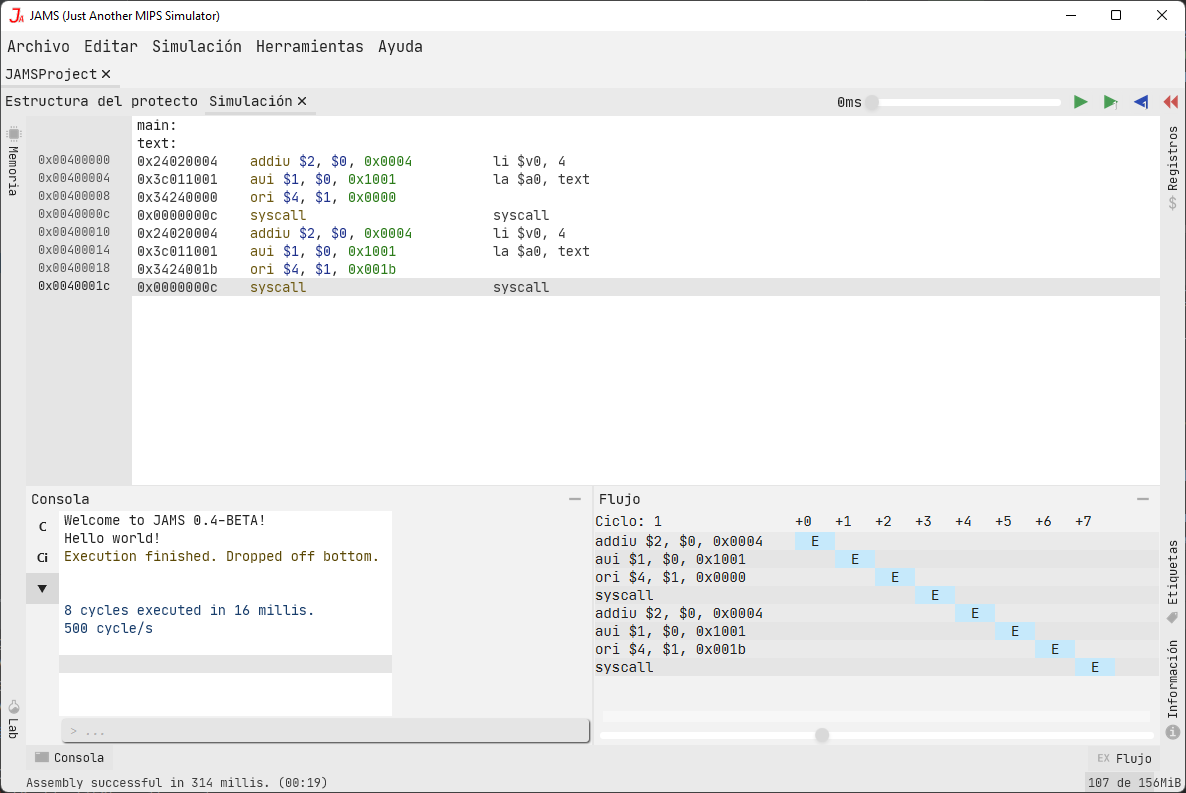
\includegraphics[width=0.8\textwidth]{images/base/jams-theme}
    \caption{\textit{JAMS} configurado para usar el modo claro}
    \label{fig:jams-light-theme}
\end{figure}


\section{Configuración}\label{sec:configuracion}

Igual que cualquier aplicación moderna, \textit{JAMS} presenta una
ventana de configuración donde el usuario podrá personalizar su experiencia.
Internamente, el sistema de configuraciones orbita
alrededor de dos archivos \textit{JSON}\cite{JSON}:
\textbf{el archivo de valores} y el \textbf{archivo de estructura}.

El archivo de valores es el encargado de almacenar los valores de
todos los \textbf{nodos} de la configuración.
Existe dos versiones de este archivo:
el primero se encuentra en la carpeta \textbf{\textasciitilde/JAMS} y representa los \textbf{valores
actuales de la configuración}.
El segundo se encuentra dentro de la propia aplicación, y es el encargado de
proporcionar \textbf{los valores por defecto de cada nodo}.
Un componente podrá agregar nuevos valores a este archivo.

\begin{lstlisting}[frame=single,label={lst:main_config.json}]
{
    "language": {
        "default": "English",
        "selected": "English"
    }
}
\end{lstlisting}

El archivo de estructura o metadatos contiene información
relacionada sobre\note{Óscar: ``relacionada sobre'' no mola} el propio nodo: el \textbf{tipo}, \textbf{región}
y \textbf{nombre} de cada nodo están definidos en este archivo.
Las secciones también tienen sus propios metadatos, especificando
el \textbf{nombre} de la sección y sus \textbf{regiones} con sus
\textbf{prioridades}.

\begin{lstlisting}[frame=single,label={lst:main_config_meta.json}]
{
    "language": {
        "meta": {
            "language_node": "CONFIG_LANGUAGE",
            "regions": {
                "language": 0
            }
        },
        "default": {
            "type": "language",
            "language_node": "CONFIG_LANGUAGE_DEFAULT",
            "region": "language"
        },
        "selected": {
            "type": "language",
            "language_node": "CONFIG_LANGUAGE_SELECTED",
            "region": "language"
        }
    }
}
\end{lstlisting}

\subsection{Interfaz de la configuración}\label{subsec:interfaz-de-la-configuración}

Para evitar que los usuarios tengan que modificar los valores de la configuración
externamente, se ha implementado una interfaz que permite modificar los
parámetros al vuelo dentro de la aplicación.
Esta interfaz es accesible directamente en la ventana de inicio o accediendo a ella
mediante la opción \textbf{Archivo > Configuración}.

Una vez la interfaz está abierta, el usuario encontrará dos nodos principales:
la lista de secciones y el visualizador de secciones.
La lista de secciones es un explorador que muestra todo el árbol de
secciones presente actualmente en la configuración.
Hay algunas secciones que contienen sub-secciones, las cuales se pueden
mostrar expandiendo la sección padre en la lista.
El visualizador de secciones muestra todos los parámetros de configuración
presentes en la sección seleccionada en la lista.
Esta interfaz aprovecha los metadatos proporcionados por el archivo
de estructura para proporcionar una interacción adecuada entre el usuario
y los diferentes parámetros.
La interfaz es extensible, pudiendo los componentes añadir nuevos tipos de datos.
La sección seleccionada puede tener un tipo de vista especial
que modifique el aspecto general del visualizador de secciones.
Es el caso de las secciones de componentes y de acciones.

\begin{figure}[H]
    \centering
    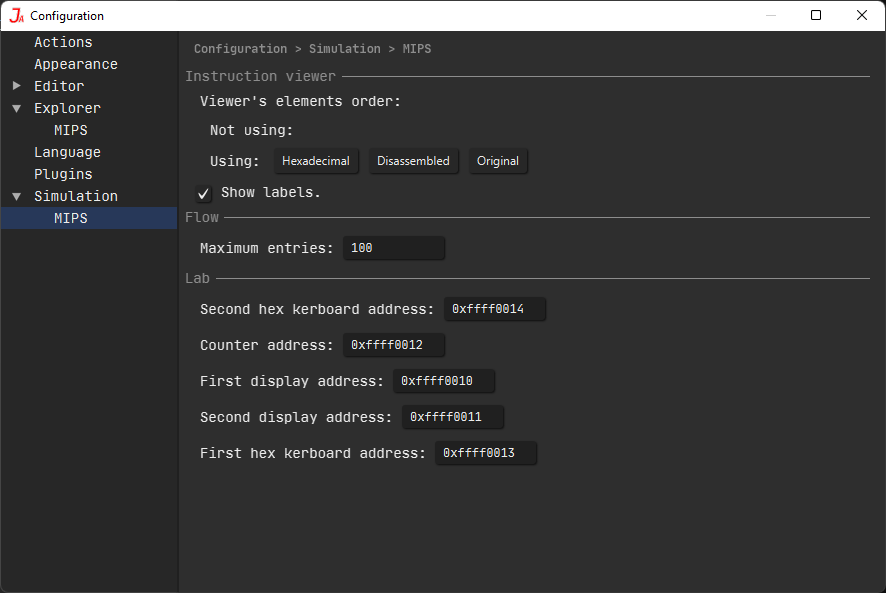
\includegraphics[width=0.8\textwidth]{images/base/jams-config}
    \caption{\textit{Interfaz de configuración}}
    \label{fig:jams-configuracion}
\end{figure}

\subsection{Secciones especiales}\label{subsec:secciones-especiales}

La interfaz de la configuración permite que ciertas gestiones se
gestionen de manera externa por un controlador diferente al \delODR{de}\newODR{establecido}
por defecto.
Estas secciones tienen una estructura totalmente diferente a la
del resto de secciones, lo que permite al usuario modificar
de manera más eficiente sus parámetros.

\section{Acciones}\label{sec:acciones}

Las acciones representan tareas que un usuario puede realizar de manera
\textbf{atómica}.
Las acciones pueden invocarse de diferentes maneras:
desde el menú principal, desde un menú de contexto
o usando una combinación de teclas modificable.
Cabe destacar que las acciones son \textbf{sensibles al contexto}:
una acción solo se podrá ejecutar en un determinado contexto
de la aplicación (el usuario no puede copiar un trozo de texto
en el explorador).

Los componentes pueden implementar nuevas acciones
creando una nueva clase que extienda $Action$ o $ContextAction$.
La clase $Action$ es la clase básica para las acciones.
Las implementaciones deben implementar \note{Óscar: ``Las implementaciones deben implementar'' no mola} el funcionamiento
de la acción en el método $run$.
La clase $ContextAction$ permite que la acción sea
mostrada en un menú contextual.
Las implementaciones de esta clase deben implementar
muchos más métodos que proporcionan información
sobre la viabilidad de la acción en diferentes contextos.

Los usuarios pueden modificar los atajos de teclado
asociados a una acción en el apartado \textbf{Acciones} de la
configuración.
Una acción puede estar vinculada a más de un atajo de teclado,
lo que le da más libertad de personalización al usuario.
La ventana de acciones contiene una barra de búsqueda que
permite buscar acciones de entre las decenas disponibles.

\begin{figure}[H]
    \centering
    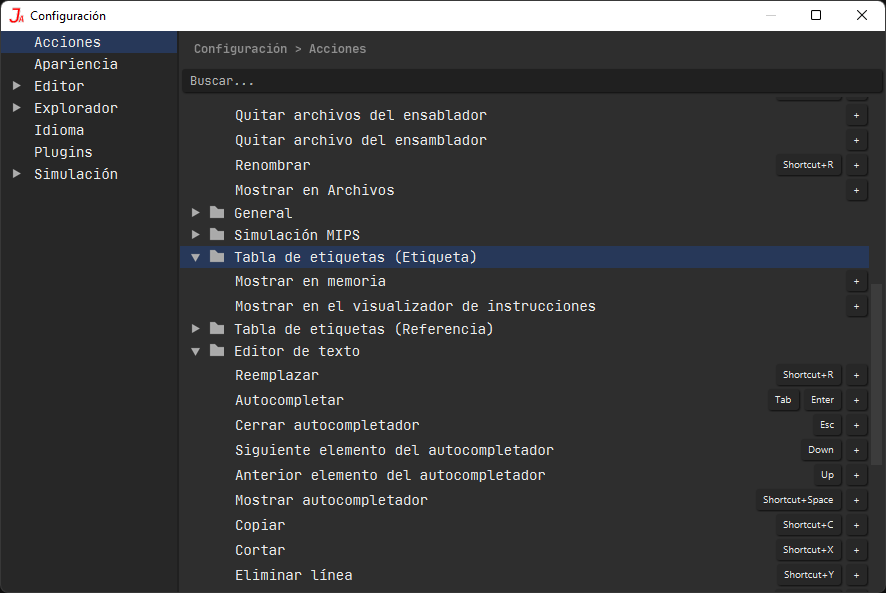
\includegraphics[width=0.8\textwidth]{images/base/jams-config-actions}
    \caption{\textit{Sección de acciones}}
    \label{fig:jams-configuracion-acciones}
\end{figure}

\section{Editor de texto}\label{sec:editor-de-texto}

El editor de texto es la tecnología que más iteraciones
ha sufrido en todo el desarrollo de \textit{JAMS},
siendo uno de los elementos más avanzados de toda
la aplicación.
El editor de texto presenta una arquitectura
\textbf{asíncrona}, y permite gestionar una gran
cantidad de líneas de texto sin bloquear la aplicación.

\subsection{Arquitectura}\label{subsec:arquitectura}

El editor de texto presenta una arquitectura
\textbf{Modelo-Vista-Controlador}:
\begin{itemize}
    \item \textbf{Vista:} la vista está gestionada
    por la librería \textit{RichTextFX}\cite{RICH_TEXT_FX}.
    \textit{RichTextFX} permite añadir estilos
    a secciones del texto.
    La vista está representada por la clase
    $CodeArea$.
    \item \textbf{Controlador:} el controlador está
    gestionado por la clase $CodeFileEditor$.
    Esta clase extiende $CodeArea$, y es la
    encargada de gestionar las entradas del usuario.
    \item \textbf{Modelo:} el modelo está representado
    por la clase $EditorIndex$.
    Las implementaciones de esta clase contienen
    una representación abstracta de los contenidos
    del editor de texto.
    El modelo se actualiza de manera asíncrona.
\end{itemize}

\subsection{Filosofía del modelo}\label{subsec:filosofía-del-modelo}

\note{Óscar: hablar de esta parte}
Debido a la gran complejidad de la arquitectura,
se ha definido una filosofía en el desarrollo
del modelo:
\begin{itemize}
    \item \textbf{Basado en elementos}: cada elemento representa
    un componente en el editor: un comentario, una instrucción,
    una etiqueta, etc.
    Los elementos son \textbf{casi inmutables}:
    solo sus inspecciones, alcances, y posición son mutables.
    \item Los elementos son recreados siempre que una línea
    es editada.
    \item Los elementos almacenan la mínima información
    posible.
    Esta información debe ser buscada usando los métodos
    de consulta proporcionados por el modelo.
    \item Los métodos de consult deben ser lo más rápidos
    posible.
    Las implementaciones por defecto utilizan la
    \textit{Stream API}\cite{STREAM_API} añadida en \textit{Java 8}.
\end{itemize}

$EditorIndexedElement$ es la la interfaz principal
que representa un elemento.
Esta interfaz define los elementos de posición, tamaño, alcance,
jerarquía y contenido.
Los elementos concretos deben implementar esta interfaz.
Una implementación básica de un elemento puede encontrarse
en la clase $EditorIndexedElementImpl$.

Si un elemento desea ser referenciado, este debe
implementar la interfaz $EditorReferencedElement$.
Un elemento que implemente esta interfaz será gestionado
de manera diferente por el modelo.
De igual manera, si un elemento desea referenciar
otros elementos, este debe implementar la interfaz
$EditorReferencingElement$.
Estas dos interfaces no son incompatibles:
un elemento puede referenciar y ser referenciado
al mismo tiempo.

El modelo es un componente \textit{thread-safe}.
Para interactuar con él, un hilo debe reservar el acceso
al modelo y especificar si desea editar su estructura o
solo acceder a sus datos.
Si el hilo modifica el modelo, se crearán dos eventos de tipo
$IndexFinishEditEvent$ y $IndexRequestRefreshEvent$
cuando termine la edición.

\subsection{Actualización del modelo}\label{subsec:actualizacion-del-modelo}

Cuando el controlador sigue el siguiente
protocolo cuando este recibe peticiones de modificación
por parte del usuario:\note{Óscar: mucho ``cuando''}
\begin{itemize}
    \item \textbf{Recolección:} las peticiones cercanas
    en el tiempo son registradas en una lista de peticiones.
    Esta lista es es procesada cuando el usuario deje
    de enviar modificaciones.
    \item \textbf{Compresión:} se descartan las peticiones
    de modificación que no van a tener efecto en el modelo.
    El caso más común de modificaciones sin efecto sería
    el de una cadena de modificaciones en una misma línea:
    solo el estado de la línea en la modificación final
    tendrá efecto en el modelo.
    \item \textbf{Actualización:} se genera una tarea
    asíncrona que modifica el modelo en base a las
    peticiones.
    \item \textbf{Finalización:} una vez \newODR{se ha modificado} el modelo
    \delODR{es modificado}, se envían una serie de eventos
    a la vista para que esta actualice el estilo
    de las líneas visibles.
\end{itemize}

\subsection{Estructura del modelo}\label{subsec:estructura-del-modelo}

El modelo presenta una arquitectura jerárquica de elementos:
un elemento tiene un padre y puede tener varios hijos.
Cada elemento contiene su posición inicial en el archivo, la
longitud de su representación y la representación en sí.
Esta estructura puede considerarse una implementación de un
\textit{Rope}\cite{ROPES}, una estructura de da\delODR{s}tos muy
utilizada para editores de texto.

\begin{center}
    \basictree{
        [Instruction 0 13 sw \$s0 0(\$s2)
        [Mnemonic 0 2 sw]
        [Parameter 3 3 \$s0
        [Register 3 3 \$s0]
        ]
        [Parameter 7 6 0(\$s2)
        [Immediate 7 1 0]
        [Register 9 3 \$s2]
        ]
        ]
    }
\end{center}

Los nodos hoja pueden implementar la interfaz
$EditorIndexStyleableElement$, permitiendo inyectar
estilos en la vista del editor de texto.
Esta interfaz solo presenta un método que pide una lista
de estilos.
\textit{JAMS} es el encargado de inyectar dichos estilos
en el editor cuando sea necesario.
El resultado puede observarse en la figura \ref{fig:jams-editor-texto}.

\begin{figure}[h]
    \centering
    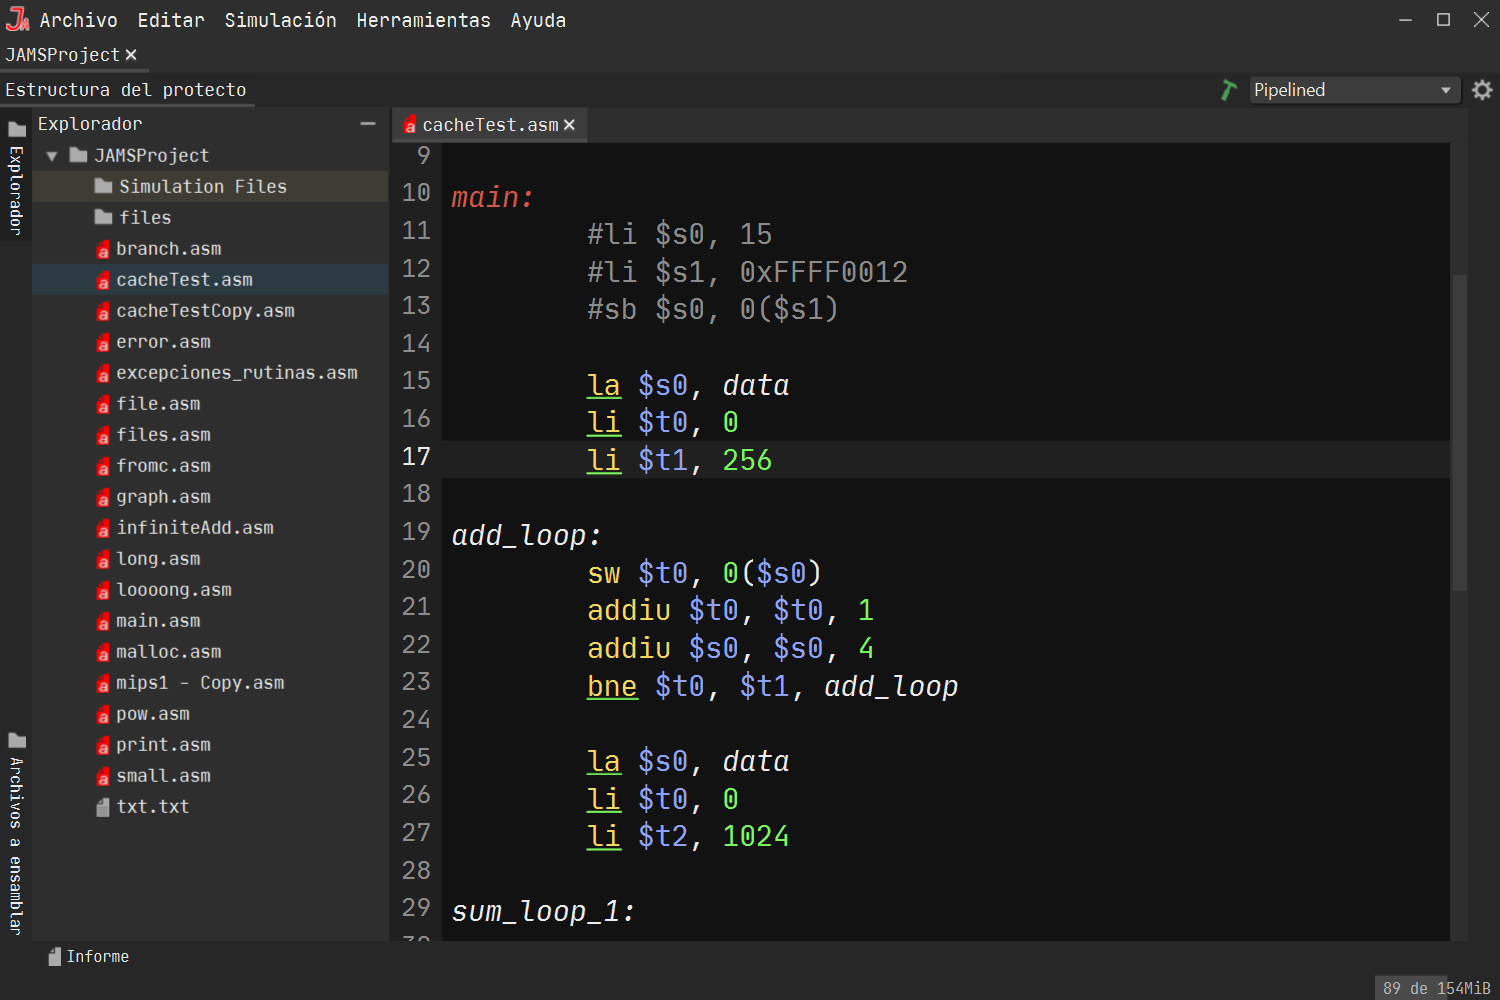
\includegraphics[width=0.8\textwidth]{images/base/jams-text-editor}
    \caption{Editor de texto con estilos inyectados}
    \label{fig:jams-editor-texto}
\end{figure}

\subsection{Referencias entre modelos}\label{subsec:referencias-entre-modelos}

Un modelo puede tener \textbf{referencias a elementos
presentes en otros modelos}.
Este es el caso de las etiquetas y macros globales.
La clase $ProjectGlobalIndex$ permite la
comunicación entre modelos, actuando de intermediador.
Solo los elementos que están dentro de los archivos
de la lista de archivos a ensamblar serán tomados en cuenta.
Para evitar interbloqueos, todas las modificaciones
realizadas en un proyecto son gestionadas en el
mismo hilo.

\subsection{Implementaciones}\label{subsec:implementaciones}

\textit{JAMS} incorpora implementaciones básicas de los
diferentes componentes usados en el editor.
Una de las implementaciones más importantes es la que está
definida en la clase $EditorLineIndex$, la cual
implementa un modelo donde cada línea representa una
unidad autocontenida.

Otras implementaciones serían la de elementos
básicos y comunes en diferentes lenguajes ensamblador:
las etiquetas, las macros, las llamadas a macros o
los comentarios son ejemplos de elementos ya definidos.

\subsection{Autocompletación}\label{subsec:autocompletacion}

\textit{JAMS} aprovecha los datos proporcionados por
el modelo para implementar una interfaz de autocompletación
que el usuario puede usar en el editor.
Esta interfaz tiene por defecto el estilo mostrado en la figura \ref{fig:jams-autocompletador}.

\begin{figure}[h]
    \centering
    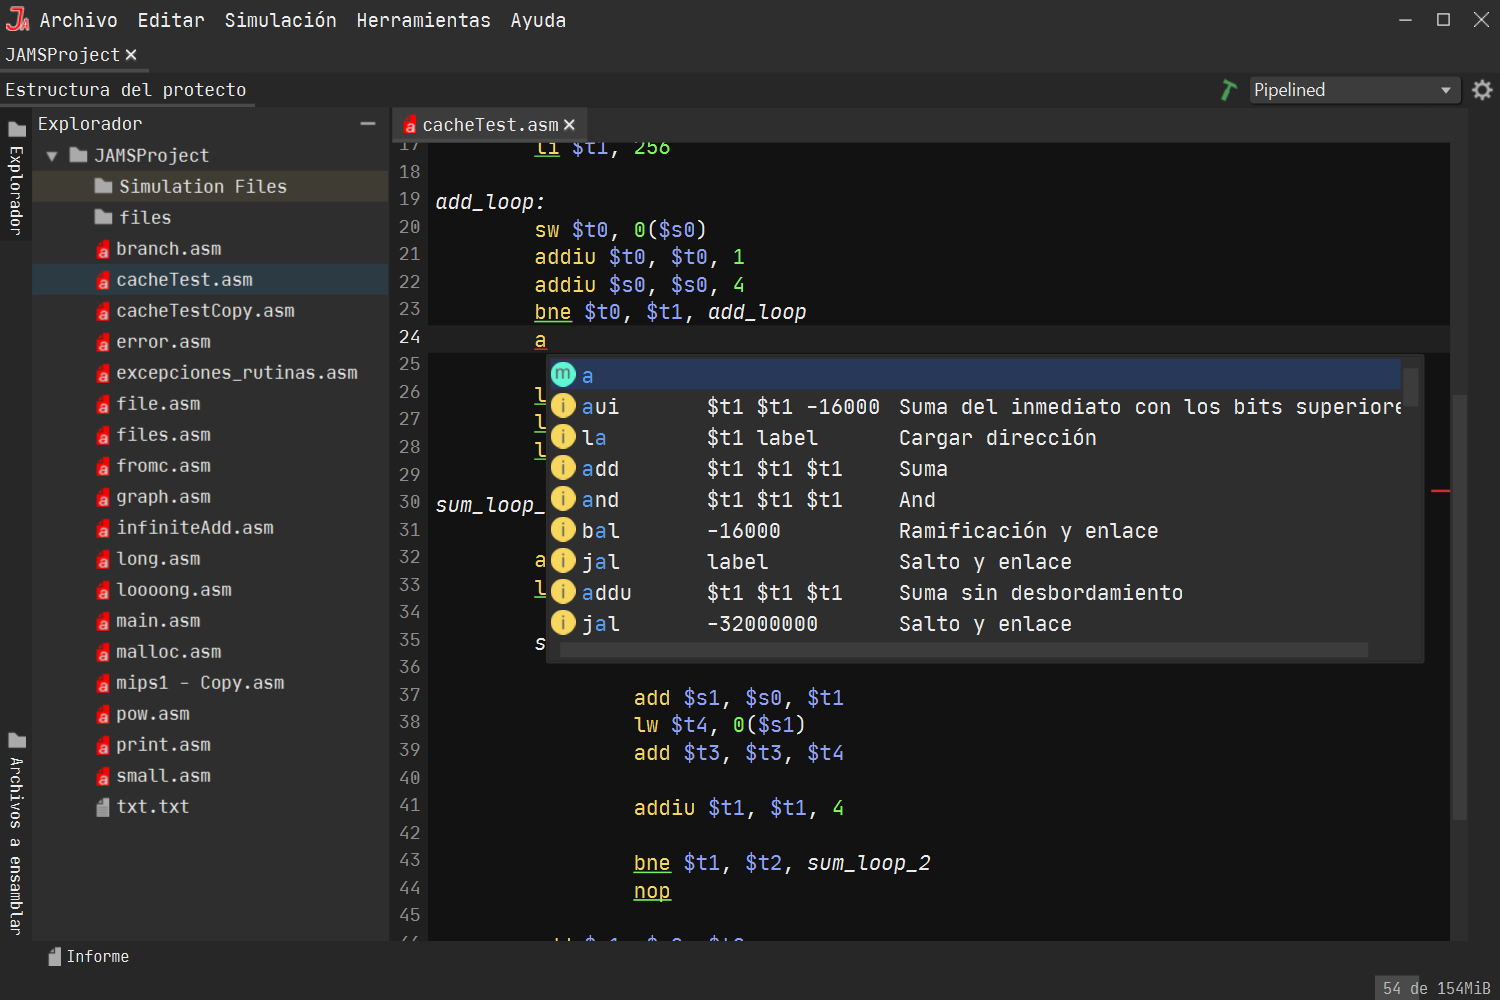
\includegraphics[width=0.8\textwidth]{images/base/jams-autocompletion}
    \caption{Autocompletador del editor de texto}
    \label{fig:jams-autocompletador}
\end{figure}

Igual que el propio editor de texto, esta interfaz
presenta una estructura modelo-vista-controlador:

\begin{itemize}
    \item \textbf{Controlador:} implementado en dos partes.
    \textit{JAMS} implementa las acciones de la interfaz,
    mientras que el desarrollador debe implementar el
    generador del modelo.
    \item \textbf{Modelo:} contiene los candidatos de
    la interfaz.
    \item \textbf{Vista:} implementa la interfaz que
    muestra los candidatos del modelo.
    \textit{JAMS} implementa una vista por defecto,
    pero los desarrolladores pueden implementar una
    vista propia.
\end{itemize}

\subsection{Documentación}\label{subsec:documentacion}

Como característica final, el editor de texto presenta
una interfaz de documentación que los proyectos
pueden utilizar para documentar sus diferentes
elementos.
Se puede acceder a la documentación con la secuencia por defecto
\textbf{Ctrl + Q}, como se puede observar en la figura \ref{fig:jams-documentacion}.

\begin{figure}[h]
    \centering
    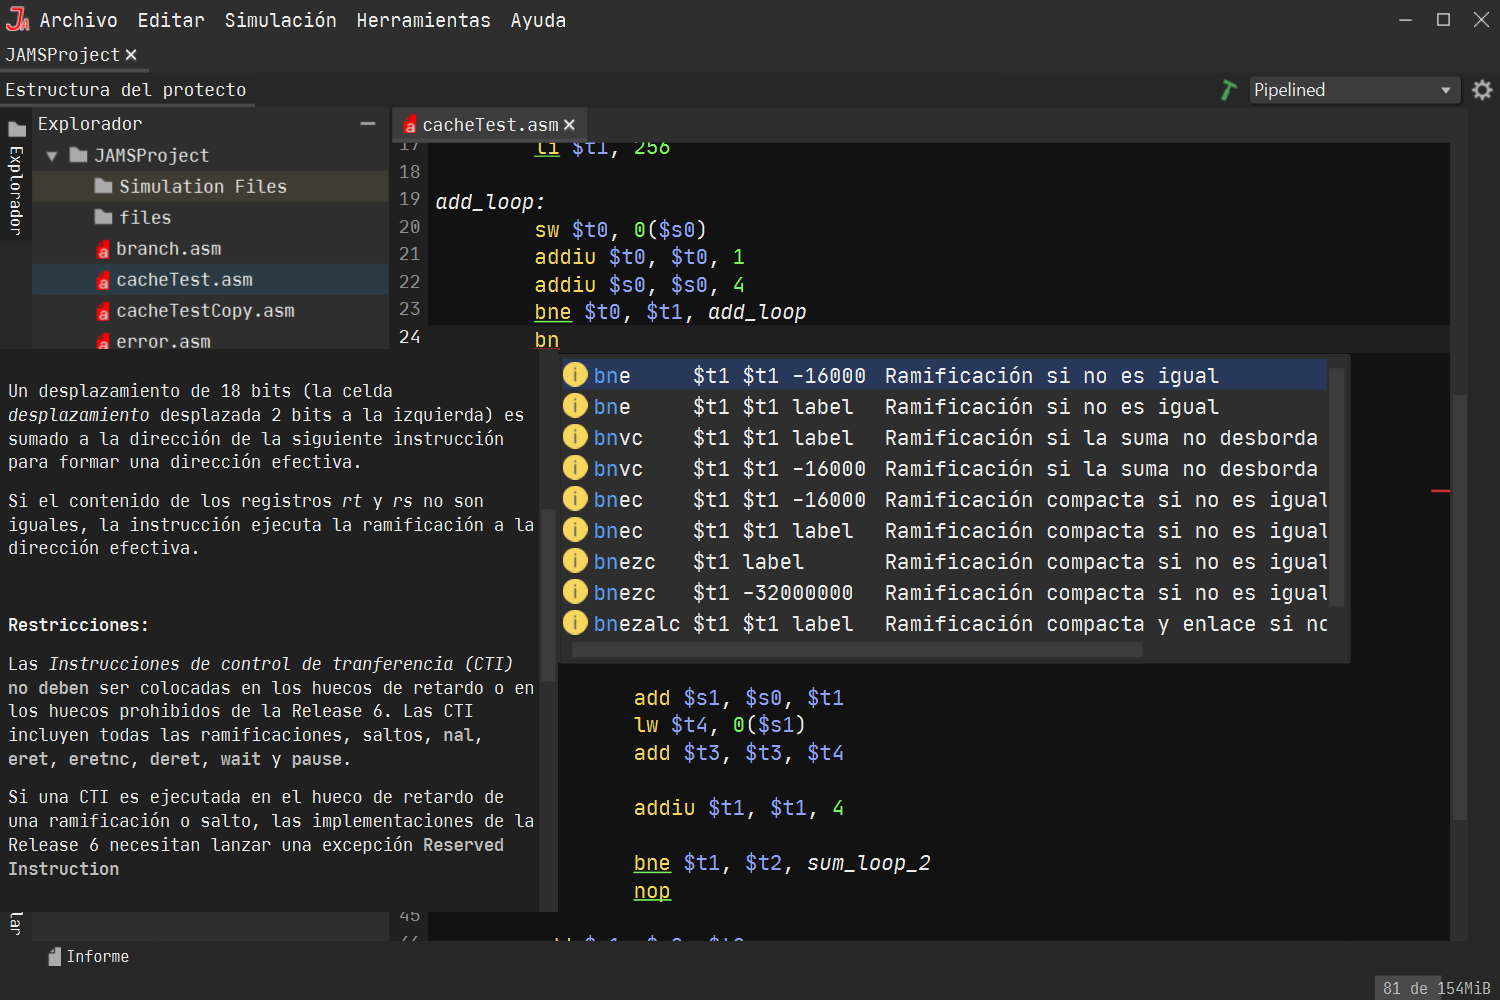
\includegraphics[width=0.8\textwidth]{images/base/jams-documentation}
    \caption{Documentación en el editor de texto}
    \label{fig:jams-documentacion}
\end{figure}
